\documentclass{scrbook}
\usepackage{graphicx} % Required for inserting images
\usepackage{tabularx} % Required for fixed width tables
\usepackage{scrlayer-scrpage} % Required for the subtitles
\usepackage{url} % Required for the URLs
\usepackage{hyperref} % Required for the URLs
\usepackage{listings} % Required for the code snippets
\usepackage{mathtools} % Required for the system of equations
\usepackage{amsmath,amssymb} % Required for some math symbols
\usepackage{enumitem} % Required for lettered lists

% Put the caption of the snippets at the bottom and allow math symbols usage
\lstset{
    captionpos=b,
    mathescape=true,
    escapeinside={(*@}{@*)}
}

% Required for circled numbers
\usepackage{tikz}
\newcommand*\circled[1]{\tikz[baseline=(char.base)]{
            \node[shape=circle,draw,inner sep=2pt] (char) {#1};}}


\title{Smart contracts}
\subtitle{Ambient intelligence course (A.Y. 2025/2026)\\Topic taught by Prof. Arnaldo Tomasino}
\author{Gabriele Colapinto}
\date{\today}

\begin{document}

\maketitle
\thispagestyle{empty}

{\Large\textbf{License}} \\
{Notes from Ambient intelligence (A.Y. 2025/2026) by Gabriele Colapinto. 
Course taught by professors Michele Ruta, Floriano Scioscia, Arnaldo Tomasino, Davide Loconte — 
Licensed under CC BY-NC 4.0.\\
\url{https://creativecommons.org/licenses/by-nc/4.0/}}

\vspace*{\fill}
\rule{\textwidth}{0.2pt}
\small{© 2025 Gabriele Colapinto \\
Released under the \href{https://creativecommons.org/licenses/by-nc/4.0/}{Creative Commons Attribution–NonCommercial 4.0 International License}}

\clearpage

\tableofcontents

\chapter{Defining the Smart Contract}

The concept of a "smart contract" significantly predates blockchain technology, yet it is within the blockchain ecosystem that the idea has found its most powerful and practical implementation. The term was first coined in 1994 by computer scientist and cryptographer Nick Szabo, who provided a foundational definition that remains relevant today: \textit{"A computerized transaction protocol that executes the terms of a contract"}.\\

Szabo envisioned a way to embed contractual clauses into hardware and software, making a breach of contract expensive, if not impossible. The general objectives of this concept were to:

\begin{itemize}
    \item Translate common contractual terms (such as payment conditions, liens, and confidentiality) into self-enforcing code.
    \item Embed them into property (hardware or software) that can self-enforce them;
    \item Minimize both malicious and accidental exceptions to the contract's execution.
    \item Reduce the need for trusted intermediaries like lawyers, brokers, and escrow agents.
\end{itemize}

The related economic goals were equally ambitious, aiming for a significant reduction in transaction costs by lowering:

\begin{itemize}
    \item Fraud loss.
    \item Arbitration and enforcement costs.
    \item Other associated transaction costs.
\end{itemize}

While the concept was revolutionary, it lacked a suitable environment for secure execution until the advent of blockchain and distributed ledger technology.

\section{Smart Contracts in a Blockchain Context}

In the context of a blockchain or distributed ledger, a smart contract is a script that is stored, verified, and executed on the distributed ledger. It can be thought of, by analogy, as a \texttt{stored procedure} in a traditional relational database.\\

Because the smart contract resides on the ledger, it is assigned a unique address. A user can trigger the execution of a smart contract by sending a transaction containing specific data to that address. Upon being triggered, the contract executes independently and automatically on a virtual machine (VM) that is running on every node in the network. The outcome of the execution is then recorded on the blockchain, and all nodes must reach a consensus on this outcome. In essence, the entire blockchain network acts as a single, distributed virtual machine responsible for the secure and reliable execution of smart contract code.

\chapter{Core Properties and an Illustrative Example}

Blockchain-based smart contracts possess a unique set of properties that enable their function as autonomous, trustworthy agents on a distributed network.

\begin{itemize}
    \item \textbf{Stateful:} A smart contract can maintain its own internal state, which is recorded on the distributed ledger. This allows it to keep track of information and change its behavior over time based on interactions.
    \item \textbf{Asset Custody:} It can hold and control on-chain digital assets (like cryptocurrencies) at its own address, much like a regular user account. It can send and receive these assets according to its pre-defined rules.
    \item \textbf{Business Logic as Code:} It allows for the direct expression of complex business rules, processes, and agreements in a high-level programming language.
    \item \textbf{Deterministic:} A smart contract is guaranteed to produce the same output for the same input every time it is executed. This property is crucial, as the network's nodes would be unable to reach consensus on the outcome of a non-deterministic execution. Nondeterministic smart contracts should be either impossible to write due to programming language \texttt{intended} design limitations or rejected on deployment.
    \item \textbf{Exhaustive Logic:} A properly written smart contract should describe all possible outcomes for any given input.
    \item \textbf{Transparent:} The code of a smart contract is stored publicly on the blockchain and can be inspected by any participant in the network.
    \item \textbf{Verifiable:} All interactions with a smart contract are recorded as cryptographically signed transactions on the blockchain. This creates a complete, immutable, and verifiable audit trail of all its operations.
\end{itemize}

\section{Example: An Automated Asset Trade}

To illustrate how these properties work in practice, consider a simple automated trade between two users, Alice and Bob, involving two assets, X and Y.\\

Bob begins by deploying a smart contract to the blockchain. This contract contains three functions: \texttt{deposit}, \texttt{trade}, and \texttt{withdraw}. The \texttt{deposit} and \texttt{trade} functions are written so that only Bob can call them using his key while the \texttt{trade} function is written in such a way that all users can call it. The latter function is programmed with a simple rule: for every 5 units of asset Y it receives, it will send back 1 unit of asset X.\\

The autonomous execution unfolds through a sequence of transactions:

\begin{enumerate}
    \item Bob calls the \texttt{deposit} function by sending a transaction that moves 3 units of his asset X into the custody of the smart contract.
    \item Alice, who wishes to trade, calls the \texttt{trade} function by sending a transaction with 10 units of her asset Y to the contract's address. The contract automatically executes its pre-defined logic, sending 2 units of asset X from its holdings to Alice in return.
    \item Finally, Bob calls the \texttt{withdraw} function. The contract verifies his identity via his digital signature and transfers all of its remaining assets (1 unit of X and the 10 units of Y it received from Alice) back to Bob's account.
\end{enumerate}

This simple example demonstrates how a smart contract can act as an autonomous economic agent, facilitating a trade between two parties without the need for a trusted intermediary like an exchange or escrow service.

\chapter{From Autonomous Actors to DAOs}

Because smart contracts operate as predictable and autonomous actors on the blockchain, they can be trusted to execute any logic that can be expressed as a function of on-chain data. This powerful capability gives rise to a more complex and revolutionary concept: the Decentralized Autonomous Organization (DAO). A DAO is an entity that exists on the blockchain whose rules, governance, and operational behavior are encoded entirely in a set of smart contracts.\\

A simple DAO can be illustrated with a delegation pattern. Imagine a primary smart contract, \texttt{SC1}, that performs its work by calling a secondary contract, \texttt{SC2}. The address of \texttt{SC2} is stored in a mutable part of \texttt{SC1}'s internal state. \texttt{SC1} also maintains a list of user public keys who are designated as voters. The contract's code includes a rule stating that a majority of these voters can agree to change the address of the contract that \texttt{SC1} calls. In this way, the behavior of the organization (represented by \texttt{SC1}) can be modified over time through a decentralized voting process, all governed by the immutable logic of the smart contract itself.

\chapter{Applications and Programming Languages}

Smart contracts are inherently general-purpose tools, capable of encoding a vast range of rules and processes. Their primary applications to date have centered on finance and the management of digital assets. Current major applications include:

\begin{itemize}
    \item Banking functions like automated escrow and savings accounts
    \item Decentralized marketplaces
    \item Prediction markets
    \item Automated distribution of music royalties
    \item Encoding and transfer of virtual property
\end{itemize}

\section{Programming Paradigms}

The majority of smart contracts on leading platforms are written in procedural programming languages, which specify \textit{what} has to be done and \textit{how} to achieve it through an ordered sequence of instructions. These languages can be categorized as follows:

\begin{itemize}
    \item \textbf{Purpose-built:} Languages created specifically for smart contract development, such as Ethereum's Solidity.
    \item \textbf{Existing Interpreted:} General-purpose scripting languages like JavaScript and Python.
    \item \textbf{Existing Compiled:} High-performance compiled languages like C++, Rust, and Go.
    \item \textbf{Existing Hybrid:} Languages that compile to an intermediate bytecode, such as Java and C\#.
\end{itemize}

Beyond the dominant procedural approach, researchers are exploring alternative paradigms that may offer advantages in security and clarity, including SQL-based languages, State Machines (like Automata and Petri nets), and Logic Programming.

\section{Comparing Development Approaches}

The choice of programming paradigm has significant implications for the development process. Let us use the following license contract as an example to illustrate the differences between the procedural approach and the state machine approach.

\begin{center}
    \textbf{\large{License contract}}
\end{center}

\begin{enumerate}[label=Article \arabic*:]
    \item The Licensor grants the Licensee a license to evaluate the Product.

    \item The Licensee must not publish the results of the evaluation of the Product without the approval of the Licenser; the approval must be obtained before the publication. If the Licensee publishes results of the evaluation of the Product without approval from the Licensor, the Licensee has 24 hours to remove the material.

    \item The Licensee must not publish comments on the evaluation of the Product, unless the Licensee is permitted to publish the results of the evaluation.

    \item If the Licensee is commissioned to perform an independent evaluation of the Product, then the Licensee has the obligation to publish the evaluation results.

    \item This license will terminate automatically if Licensee breaches this Agreement.
\end{enumerate}

\subsection{Procedural approach}

\begin{figure}
    \centering
    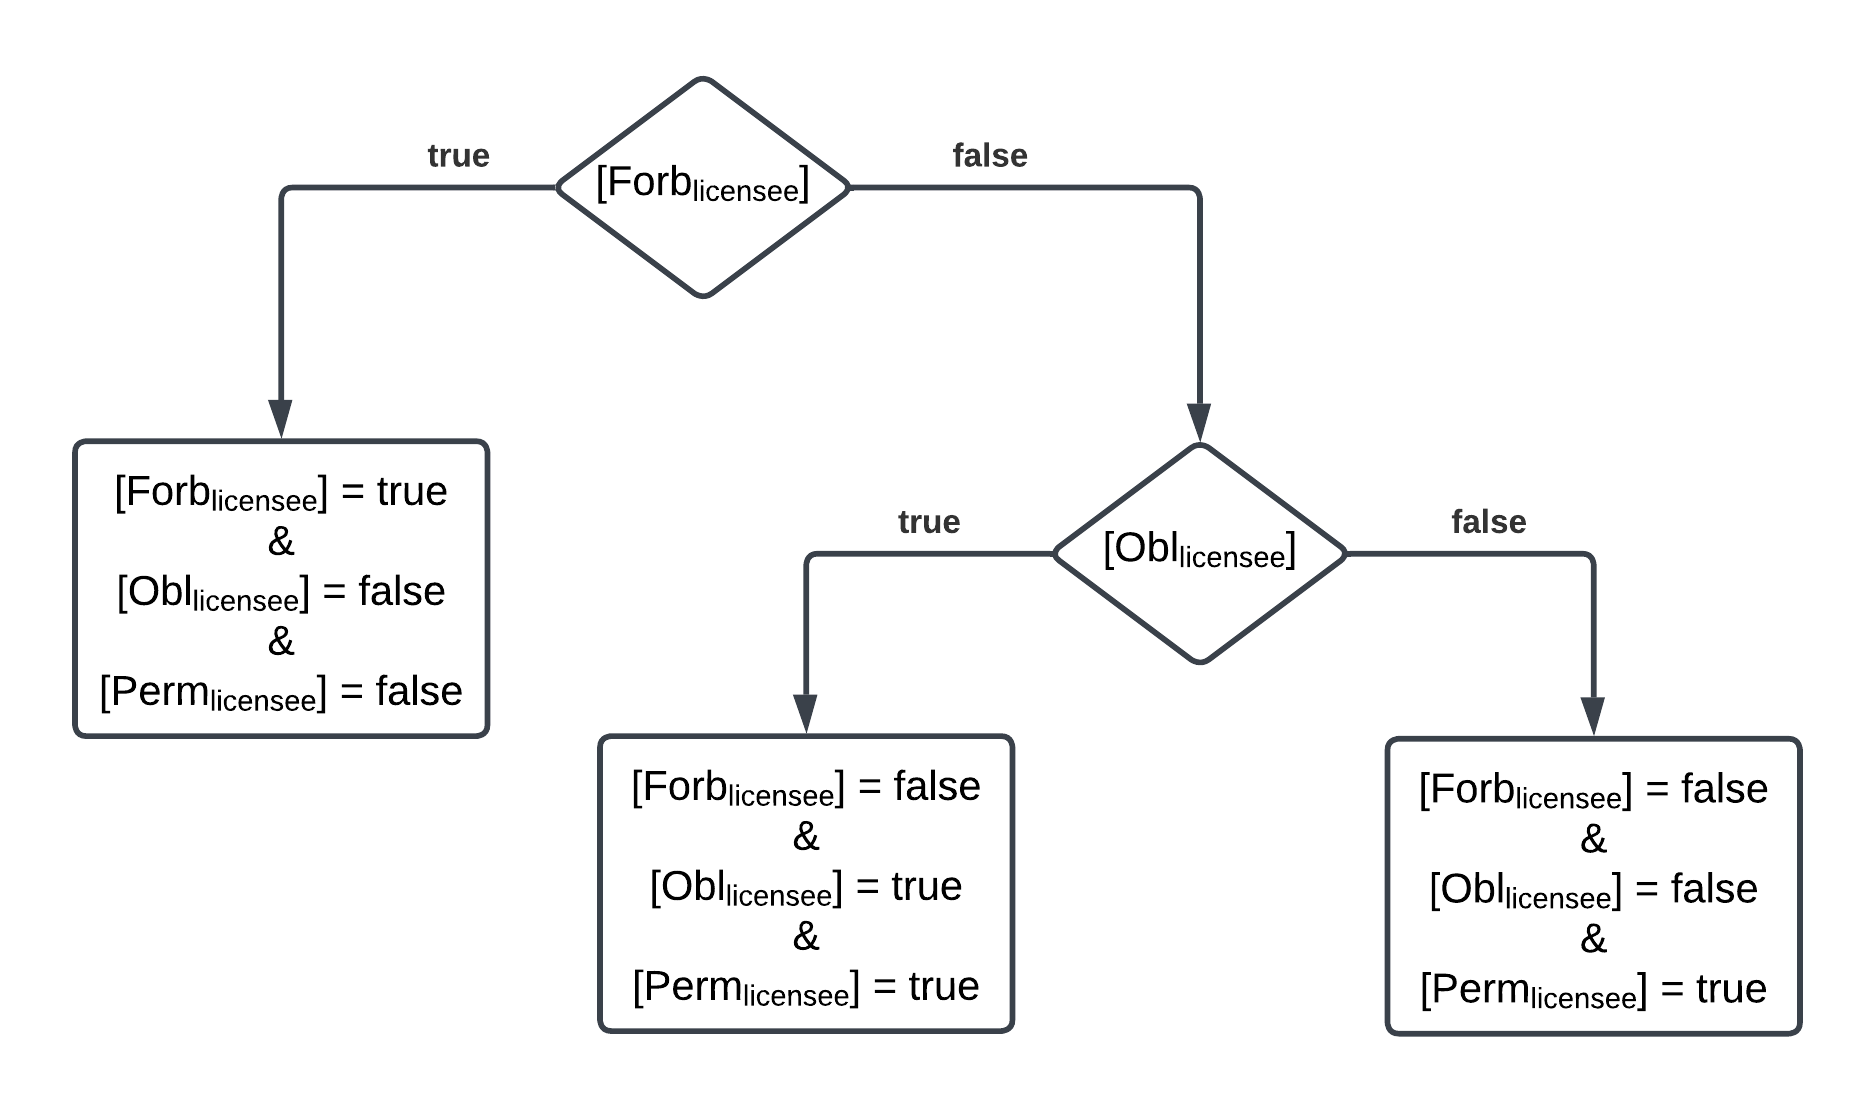
\includegraphics[width=0.5\linewidth]{Images/Pseudo_code_variable_management.png}
    \caption{Pseudo-code variable management}
    \label{fig:pseudo_code_variable_management}
\end{figure}

\begin{figure}
    \centering
    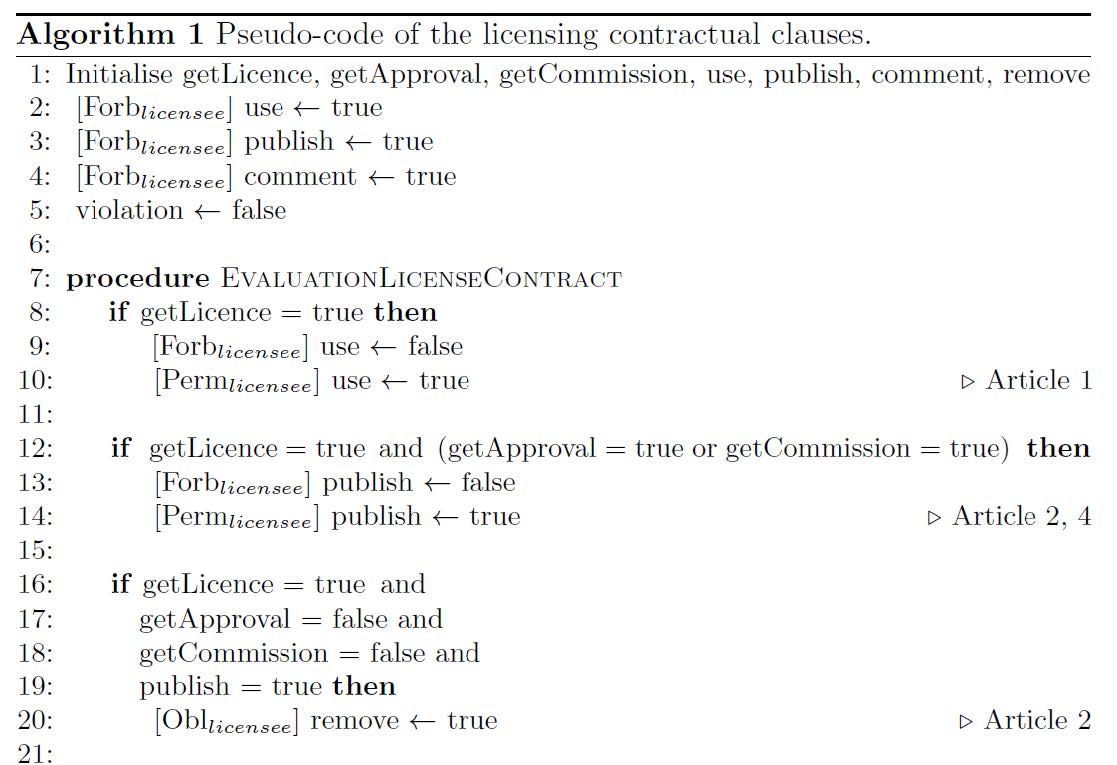
\includegraphics[width=\linewidth]{Images/Pseudo_code_1.jpg}
    \caption{License contract pseudo-code - Part 1}
    \label{fig:pseudo_code_1}
\end{figure}

To expose the procedural approach we will refer to the pseudo-code contained in figures ~\ref{fig:pseudo_code_1} and ~\ref{fig:pseudo_code_2}. \\

Before we proceed, we need to understand the way variables are designed and managed in the pseudo-code. Each variable represents an action of the licensee and it has a label that specifies its deontic modality: $[Forb_{licensee}]$ for forbidden, $[Obl_{licensee}]$ for obliged and $[Perm_{licensee}]$ for permitted. Figure ~\ref{fig:pseudo_code_variable_management} shows how the code manages the deontic modalities of the actions. One might notice that $[Forb_{licensee}]$ is used as if to say $\neg [Perm_{licensee}]$ because every time something is not forbidden it is permitted. This means that one of these modalities is redundant and can be replaced with a proper usage of the other. As for the $[Obl_{licensee}]$ modality, instead, this represents an additional and stronger condition because if something is obliged then it is not only permitted but the licensee must perform that action. Something can also be permitted but not obliged meaning that the licensee can decide to perform that action or not. \\

Now, let us expose the pseudo-code. At the beginning we have the initialization of the variables. The assumption at this point is that the licensee did not start the evaluation of the product yet so, they can't use the product, publish the results of the evaluation, publish comments on the evaluation or commit a violation of the contract. \\

At line 7 we have the declaration of the procedure that evaluates the license contract whose content is executed at every evaluation. Remember: the interaction with a smart contract is made through cryptographically signed transactions so, the licensee interacts with the smart contract by calling the functions that change the variables the developer wants to make available from the outside. In this case, the variables related to the status and the user actions with the exception of \texttt{violation} which is intended to be managed only by the business logic of the smart contract. \\

Inside the evaluation procedure we have the implementation of the articles of the contract. In lines from 8 to 10 we have the implementation of article 1 that says that if the user has a license to evaluate the product they are allowed to use it. \\

In lines from 12 to 14 we have the partial implementation of articles 2 and 4 which both state that a user is allowed to publish the results of the evaluation but under different conditions. The requirement of the article 2 is that the user gets the approval of the Licenser while the requirement of the article 4 is that the user is commissioned to evaluate the product. From lines 16 to 20 we have the implementation of the rest of article 2. \texttt{Notice that this implementation of the smart contract can only establish that the user is obliged to remove the published data but does not check if the data was actually removed within 24 hours from the infringement.} Smart contracts are transactional systems and cannot change state by themselves using a timer but the programmer can implement a business rule that records the timestamp of the infringement and checks if the removal of the result data was made within 24 hours from the latter. \\

\begin{figure}
    \centering
    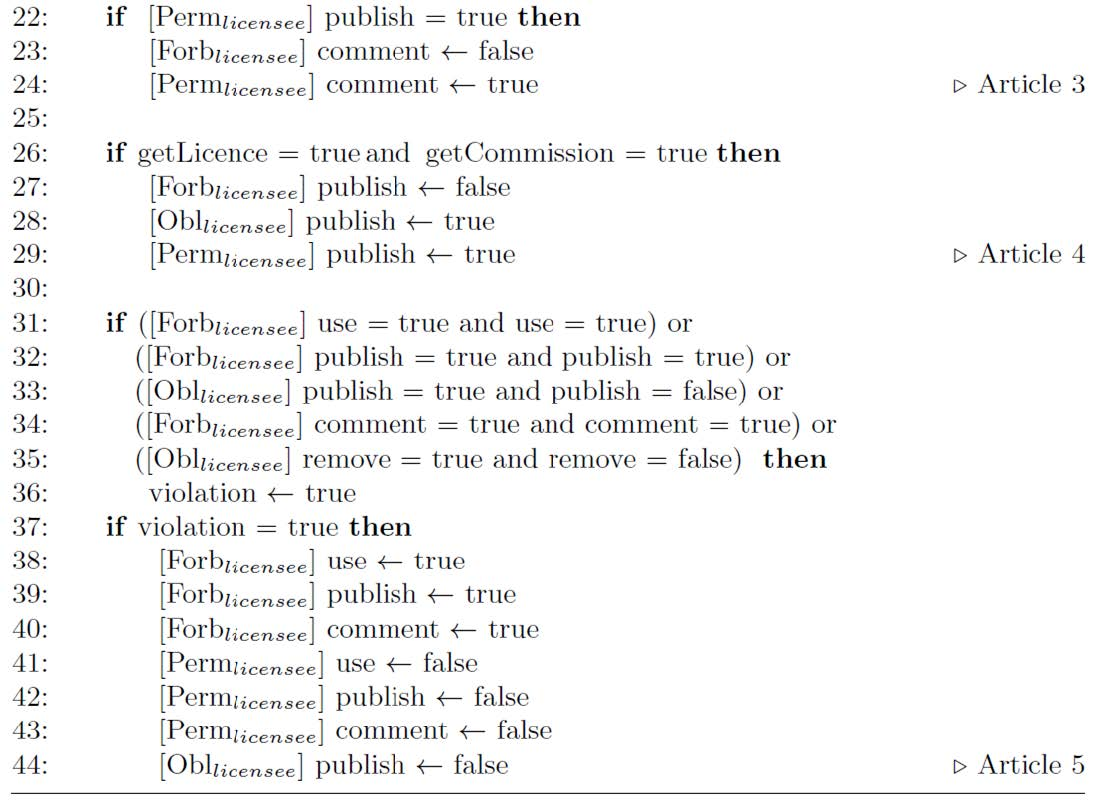
\includegraphics[width=\linewidth]{Images/Pseudo_code_2.jpg}
    \caption{License contract pseudo-code - Part 2}
    \label{fig:pseudo_code_2}
\end{figure}

The implementation of article 3 is simple and self-explanatory and we can find it in lines from 22 to 24. \\

From lines to 26 to 29 we can find the implementation of article 4. It is simple and self-explanatory but let us look at the condition better and compare it with the one of the first part of the implementation of article 2 at line 12. The condition of the first part of the implementation of article 2 includes the possibility of getting the permission from the commission because the second part of the implementation the code evaluates unauthorized publications of the results. This part of the code makes us understand a key shortcoming of the procedural approach: \texttt{there isn't a unique implementation for the contract}. The code could have been rewritten as follows and it would have worked the same:

\begin{lstlisting}[caption={Alternative implementation of articles 2 and 4}]
    // Article 2 condition
    if getLicense = true and getApproval = true then
        [(*@$\text{Forb}_{licensee}$@*)] publish (*@$\leftarrow$@*) false
        [(*@$\text{Perm}_{licensee}$@*)] publish (*@$\leftarrow$@*) true

    // Article 4
    if getLicense = true and getCommission = true then
        [(*@$\text{Forb}_{licensee}$@*)] publish (*@$\leftarrow$@*) false
        [(*@$\text{Obl}_{licensee}$@*)] publish (*@$\leftarrow$@*) true
        [(*@$\text{Perm}_{licensee}$@*)] publish (*@$\leftarrow$@*) true

    // Infringement detection - Second part of article 2
    if getLicense = true and
       getApproval = false and
       getCommission = false and
       publish = true then
        [(*@$\text{Obl}_{licensee}$@*)] remove (*@$\leftarrow$@*) true
\end{lstlisting}

Lines from 31 to 44 contain the implementation of article 5 which detects violations of the contract and, in case of violation, prohibits the user from using the product. Notice that there isn't another piece of code which sets \texttt{violation = false} so, the prohibition is permanent. The only thing a user can do at this point is to stipulate another contract so that the variable \texttt{violation} is initialized to \texttt{false} again.\\

In conclusion, writing procedural code for a contract can be cumbersome and highly error-prone. The programmer must manually translate legal reasoning and contractual clauses into a precise, ordered sequence of instructions. They are solely responsible for determining how events change the state of obligations and permissions and for ensuring that those changes are propagated correctly according to the contract's intended meaning. This places the burden of complex legal reasoning directly on the programmer.

\subsection{State machine approach}

\begin{figure}
    \centering
    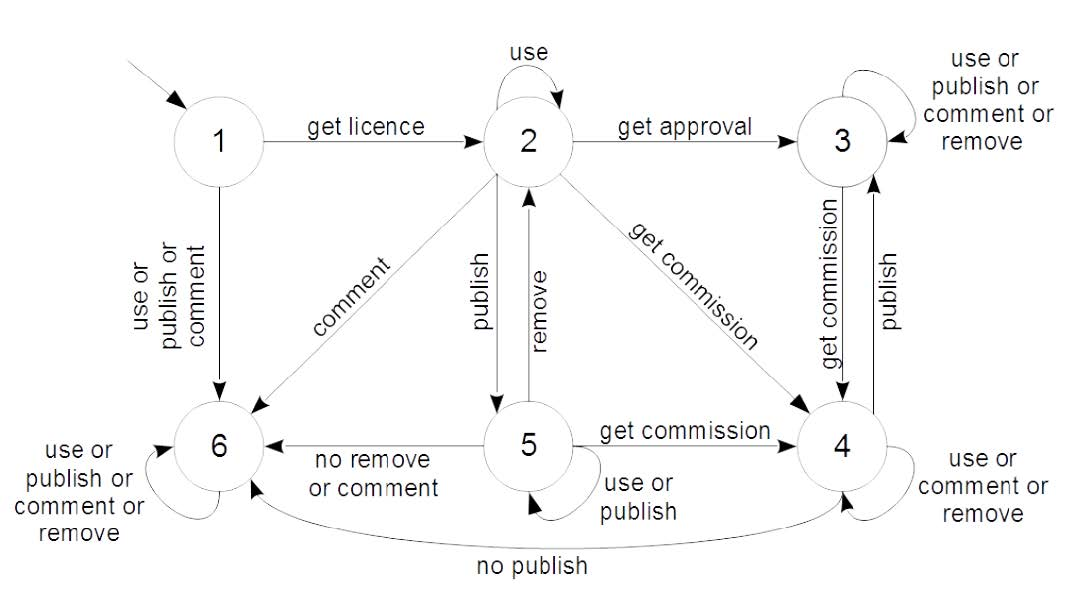
\includegraphics[width=\linewidth]{Images/State_machine.jpg}
    \caption{License contract state machine}
    \label{fig:state_machine}
\end{figure}

To expose the state machine approach we will refer to the state machine contained in figure ~\ref{fig:state_machine}. \\

Before we start the exposition it's useful to clarify that smart contracts state machines are constructed in a similar way to finite-state automata. We have an initial state which is related to an initial assumption and for each state we have a possible set of actions that can change the state the user is in. In this case, the initial assumption is that the user does not have a license to use the product and the set of possible actions is:

\begin{enumerate}
    \item get license
    \item get approval
    \item get commission
    \item use
    \item publish
    \item comment
    \item remove
\end{enumerate}

Notice that these actions are related to external user interaction with the smart contract and they are the same defined in the first line of the pseudo-code. \\

For each state we run through all the possible actions and check if they are possible in the current state. If so, we ask ourselves where would they lead if executed. If the consequence of the action is a state that does not exist, we create it. \\

Now, let us start the exposition of the smart contract state machine.

The initial state is \circled{1}. In this state the user does not have a license yet. The possible actions in this state are: \texttt{get license}, \texttt{use}, \texttt{publish} and \texttt{comment} because the other actions are not possible. In order to get the approval or to be commissioned a user must be licensed first. Furthermore, a user cannot have data to remove if they didn't publish anything yet. \\

Getting the license would make the user a licensed user and lead them to another state (\circled{2}). Using the product, publishing the usage results or commenting them would be a violation of the license contract and would lead the user to a terminal state (\circled{6}).\\

In state \circled{2} the user is licensed and can \texttt{use} the product, \texttt{publish} the evaluation result and \texttt{comment} it, get the Licenser \texttt{approval} and get the approval of the \texttt{commission}. They can't remove the published data because they didn't publish anything yet and they cannot get another license because they already have it. The sole usage of the product does not trigger any contract condition so, using the product does not result in a change of state. We represent this missed transition creating a self pointing arc in state \circled{2}. Publishing the results of the evaluation in this state would trigger the condition related to article 2, lead the user to another state in which they are obliged to remove the published data within 24 hours from the infringement. Publishing comments on the evaluation of the product would trigger the condition expressed in article 3 and result in an infringement but, in this case, the contract doesn't express a way to emend it. This means that in this case the violation of the contract leads the user into a terminal state of the state machine. If the user gets the approval of the Licenser or the commission they get in the states expressed respectively in articles 2 and 4. \\

The state \circled{3} is the state in which the user got the approval of the Licenser and is now allowed to legitimately use the product, publish its results and comments and remove all the published material at will. They cannot get another license or another approval of the Licenser because they already have both but they can still get the approval of the commission. In such case they get in another state in which they are obliged to publish the results of the evaluation as stated in article 4. \\

In state \circled{4} the user was licensed to use the product and is obliged to publish the results of the evaluation. In this state the user can use the product, comment the results of the evaluation and remove them without changing state. They cannot get a license, the approval of the Licenser or the approval of the commission because they already have them. What determines the state change in this case is the publication of the results. If it happens, the user gets into state \circled{3} and becomes a licensed user. If it doesn't, it results in a violation of the contract and the user gets into the terminal state of the state machine. \\

State \circled{4} exposes another problem of smart contracts. \textbf{Some articles can have an ambiguous interpretation.} If we read article 4 we cannot tell if, after the commissioned publication, the user becomes licensed or not. One can also interpret the approval of the commission as a single-use permission to the user. \\

State \circled{5} is about unapproved publications of results. As expressed by article 2 the user is obliged to remove the published data within 24 hours from the infringement. In this state the user cannot get a license because they already have one and they cannot get the approval of the Licenser because the latter is the one that defines what results in an infringement of the contract. Roughly speaking: if a user gets into trouble because they disobey to the Licenser, the latter does not approve that action so asking for approval after the infringement is useless.

In this state the user can use the product and publish its results without changing state. If they removed the published material, they emend the infringement and return to state \circled{2} but if they don't, it results in a violation of the contract leading the user into a terminal state.

At this point we can notice once again that there isn't a unique implementation of the contract because the developer of the state machine had to interpret the outcome of two actions which was not stated in the license contract: commenting the results of the product usage and getting the approval of the commission.

If the user comments the results of the usage they get into the terminal state but they can try to save themselves from state \circled{5} also by asking for the approval of the commission which, if happens, would lead them into state \circled{4}. \\

State \circled{6} is the terminal state of the contract. In this state the user can't get a license or get approvals from the Licenser or the commission. As for the other actions, we have another interpretation of the developer. The fact that the other operations are related to a self-pointing arc means that the developer foresaw the possibility of unlicensed interaction with the product. Another developer could have removed this possibility by not creating the self-pointing arcs allowing for sole licensed product usage. \\

 In conclusion, using a state machine can help alleviate some of these complications, particularly for large contracts, by providing a formal model to guide the creation of procedural code. However, this approach has its own limitations. For non-trivial contracts, state machines can grow exponentially large and complex. Crucially, the programmer still remains in charge of the underlying legal reasoning required to construct the state machine in the first place.

\chapter{The Legal Landscape}

A critical question surrounding this technology is its legal standing: are smart contracts legally binding? In most jurisdictions, the answer is not yet.\\

Adapting current legal systems to recognize and enforce code as a legally binding instrument is a complex and heavily debated matter among law scholars and policymakers. The challenge is further complicated by the inherent tension between the global, borderless nature of many blockchain systems and the national, jurisdiction-specific basis of contract law.\\

The path forward is not purely technical. As with many socio-technical matters, achieving real, useful, and fair progress will require continued dialogue and collaboration among experts in technology, law, and economics to bridge the gap between what is computationally possible and what is legally recognized.

\end{document}
